\documentclass[]{article}
\usepackage{lmodern}
\usepackage{amssymb,amsmath}
\usepackage{ifxetex,ifluatex}
\usepackage{fixltx2e} % provides \textsubscript
\ifnum 0\ifxetex 1\fi\ifluatex 1\fi=0 % if pdftex
  \usepackage[T1]{fontenc}
  \usepackage[utf8]{inputenc}
\else % if luatex or xelatex
  \ifxetex
    \usepackage{mathspec}
  \else
    \usepackage{fontspec}
  \fi
  \defaultfontfeatures{Ligatures=TeX,Scale=MatchLowercase}
\fi
% use upquote if available, for straight quotes in verbatim environments
\IfFileExists{upquote.sty}{\usepackage{upquote}}{}
% use microtype if available
\IfFileExists{microtype.sty}{%
\usepackage{microtype}
\UseMicrotypeSet[protrusion]{basicmath} % disable protrusion for tt fonts
}{}
\usepackage[margin=1in]{geometry}
\usepackage{hyperref}
\hypersetup{unicode=true,
            pdftitle={Pick-up method + machine learning: a proved efficient approach to forecast hotel demand},
            pdfauthor={Rachel Zhang},
            pdfborder={0 0 0},
            breaklinks=true}
\urlstyle{same}  % don't use monospace font for urls
\usepackage{graphicx,grffile}
\makeatletter
\def\maxwidth{\ifdim\Gin@nat@width>\linewidth\linewidth\else\Gin@nat@width\fi}
\def\maxheight{\ifdim\Gin@nat@height>\textheight\textheight\else\Gin@nat@height\fi}
\makeatother
% Scale images if necessary, so that they will not overflow the page
% margins by default, and it is still possible to overwrite the defaults
% using explicit options in \includegraphics[width, height, ...]{}
\setkeys{Gin}{width=\maxwidth,height=\maxheight,keepaspectratio}
\IfFileExists{parskip.sty}{%
\usepackage{parskip}
}{% else
\setlength{\parindent}{0pt}
\setlength{\parskip}{6pt plus 2pt minus 1pt}
}
\setlength{\emergencystretch}{3em}  % prevent overfull lines
\providecommand{\tightlist}{%
  \setlength{\itemsep}{0pt}\setlength{\parskip}{0pt}}
\setcounter{secnumdepth}{0}
% Redefines (sub)paragraphs to behave more like sections
\ifx\paragraph\undefined\else
\let\oldparagraph\paragraph
\renewcommand{\paragraph}[1]{\oldparagraph{#1}\mbox{}}
\fi
\ifx\subparagraph\undefined\else
\let\oldsubparagraph\subparagraph
\renewcommand{\subparagraph}[1]{\oldsubparagraph{#1}\mbox{}}
\fi

%%% Use protect on footnotes to avoid problems with footnotes in titles
\let\rmarkdownfootnote\footnote%
\def\footnote{\protect\rmarkdownfootnote}

%%% Change title format to be more compact
\usepackage{titling}

% Create subtitle command for use in maketitle
\providecommand{\subtitle}[1]{
  \posttitle{
    \begin{center}\large#1\end{center}
    }
}

\setlength{\droptitle}{-2em}

  \title{Pick-up method + machine learning: a proved efficient approach to
forecast hotel demand}
    \pretitle{\vspace{\droptitle}\centering\huge}
  \posttitle{\par}
    \author{Rachel Zhang}
    \preauthor{\centering\large\emph}
  \postauthor{\par}
      \predate{\centering\large\emph}
  \postdate{\par}
    \date{05/24/2020}

\usepackage{booktabs}
\usepackage{longtable}
\usepackage{array}
\usepackage{multirow}
\usepackage{wrapfig}
\usepackage{float}
\usepackage{colortbl}
\usepackage{pdflscape}
\usepackage{tabu}
\usepackage{threeparttable}
\usepackage{threeparttablex}
\usepackage[normalem]{ulem}
\usepackage{makecell}
\usepackage{xcolor}

\begin{document}
\maketitle

\section{Data}\label{data}

\subsection{Data Importing and
Cross-Validation}\label{data-importing-and-cross-validation}

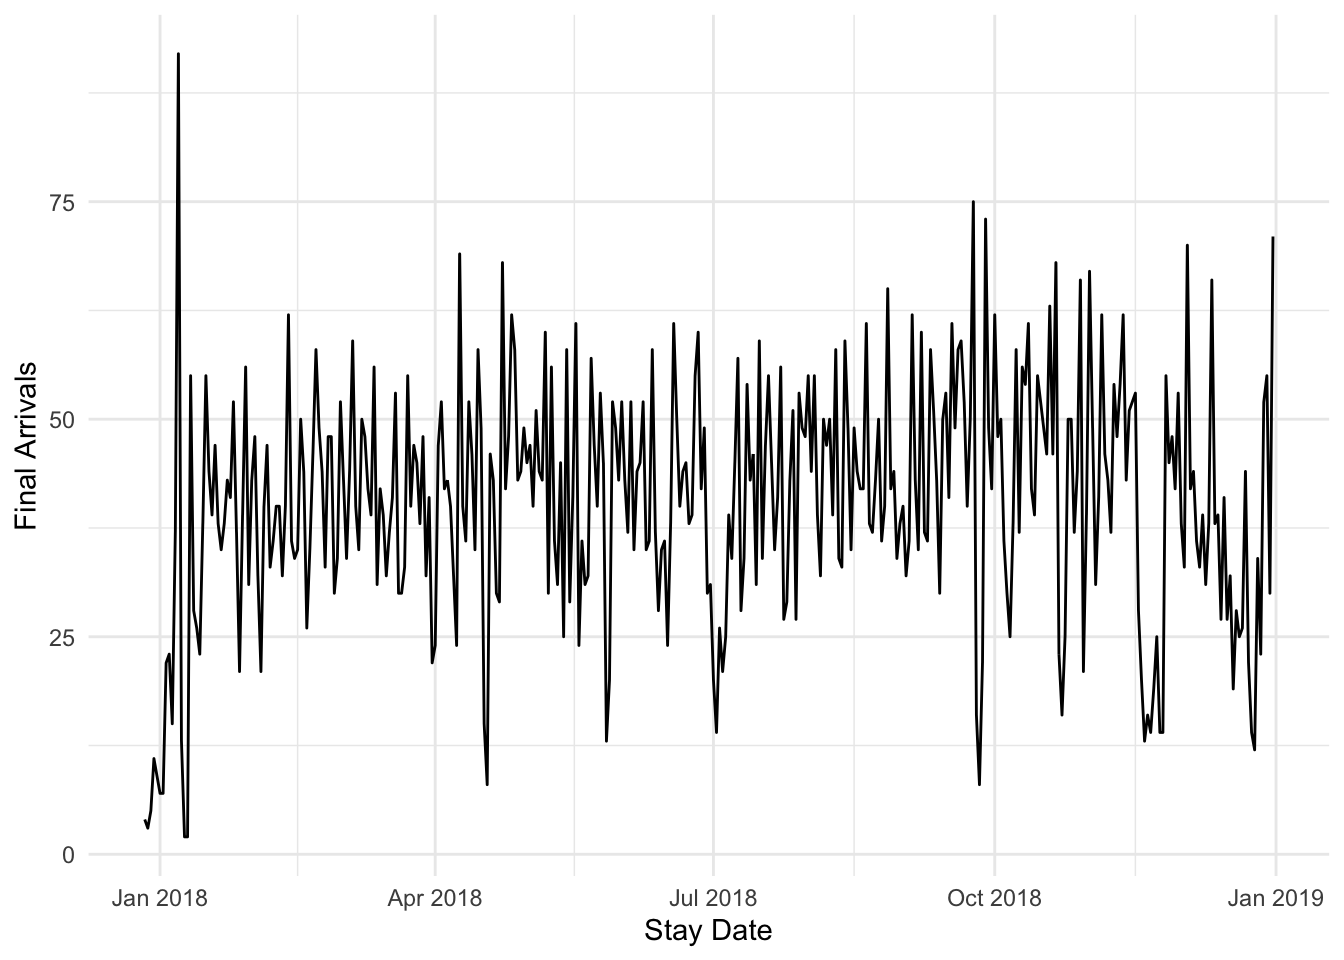
\includegraphics{ffffffffinal0524_files/figure-latex/loaddata-1.pdf}

\begin{table}[!h]

\caption{\label{tab:cv}Training Set Overview}
\centering
\resizebox{\linewidth}{!}{
\begin{tabular}{lrlrrrrrrrrrrrr}
\toprule
  & ROH0 & DOW & ROH1 & ROH2 & ROH3 & ROH4 & ROH5 & ROH6 & ROH7 & ROH14 & ROH21 & ROH30 & ROH60 & ROH90\\
\midrule
\rowcolor{gray!6}  2018-11-15 & 52 & Thursday & 49 & 46 & 42 & 41 & 41 & 41 & 38 & 29 & 25 & 22 & 7 & 1\\
2018-06-11 & 58 & Monday & 58 & 56 & 53 & 51 & 47 & 47 & 47 & 40 & 37 & 30 & 9 & 4\\
\rowcolor{gray!6}  2018-05-04 & 51 & Friday & 48 & 47 & 46 & 44 & 41 & 38 & 38 & 30 & 28 & 21 & 4 & 1\\
2018-10-21 & 68 & Sunday & 67 & 67 & 66 & 66 & 64 & 59 & 54 & 44 & 20 & 18 & 10 & 5\\
\rowcolor{gray!6}  2018-09-22 & 40 & Saturday & 38 & 36 & 36 & 35 & 33 & 32 & 31 & 27 & 20 & 8 & 5 & 5\\
\addlinespace
2018-07-01 & 20 & Sunday & 17 & 16 & 16 & 14 & 13 & 13 & 13 & 10 & 10 & 6 & 2 & 2\\
\rowcolor{gray!6}  2018-10-29 & 66 & Monday & 61 & 56 & 55 & 53 & 51 & 49 & 43 & 32 & 26 & 25 & 7 & 2\\
2018-03-21 & 30 & Wednesday & 28 & 25 & 21 & 21 & 21 & 20 & 20 & 9 & 5 & 5 & 3 & 0\\
\rowcolor{gray!6}  2018-09-29 & 49 & Saturday & 45 & 45 & 42 & 39 & 37 & 36 & 36 & 31 & 26 & 23 & 17 & 12\\
2018-11-21 & 14 & Wednesday & 14 & 13 & 12 & 12 & 12 & 12 & 11 & 10 & 10 & 9 & 6 & 2\\
\bottomrule
\end{tabular}}
\end{table}

\subsection{Modeling}\label{modeling}

\subsubsection{Additive Pick-up}\label{additive-pick-up}

\begin{table}[!h]

\caption{\label{tab:apk}Additive Pick Ups}
\centering
\resizebox{\linewidth}{!}{
\begin{tabular}{lrrrrrrrrrrrr}
\toprule
DOW & ROH1 & ROH2 & ROH3 & ROH4 & ROH5 & ROH6 & ROH7 & ROH14 & ROH21 & ROH30 & ROH60 & ROH90\\
\midrule
\rowcolor{gray!6}  Sunday & 2.11 & 3.04 & 4.40 & 5.58 & 6.51 & 8.18 & 9.22 & 13.9 & 18.8 & 22.8 & 30.1 & 33.9\\
Monday & 2.84 & 4.34 & 5.16 & 7.59 & 9.57 & 11.14 & 12.89 & 21.8 & 27.4 & 33.2 & 42.6 & 45.9\\
\rowcolor{gray!6}  Tuesday & 2.42 & 4.28 & 4.58 & 4.97 & 6.17 & 7.25 & 8.92 & 16.6 & 21.7 & 27.3 & 33.5 & 36.7\\
Wednesday & 1.95 & 3.58 & 5.37 & 5.77 & 6.16 & 7.30 & 8.51 & 15.5 & 20.5 & 25.3 & 32.6 & 35.8\\
\rowcolor{gray!6}  Thursday & 3.40 & 5.11 & 6.84 & 8.31 & 8.84 & 9.67 & 10.84 & 17.0 & 21.4 & 25.8 & 34.1 & 37.3\\
\addlinespace
Friday & 3.32 & 5.76 & 7.61 & 9.27 & 10.83 & 11.54 & 12.24 & 17.9 & 21.6 & 25.5 & 33.6 & 37.5\\
\rowcolor{gray!6}  Saturday & 3.71 & 5.69 & 7.74 & 9.55 & 10.98 & 12.14 & 12.88 & 17.3 & 20.3 & 23.7 & 30.3 & 33.3\\
\bottomrule
\end{tabular}}
\end{table}

\subsubsection{Multiplicative Pick-up}\label{multiplicative-pick-up}

\begin{table}[!h]

\caption{\label{tab:mpk}Multiplicative Pick Ups}
\centering
\resizebox{\linewidth}{!}{
\begin{tabular}{lrrrrrrrrrrrr}
\toprule
DOW & ROH1 & ROH2 & ROH3 & ROH4 & ROH5 & ROH6 & ROH7 & ROH14 & ROH21 & ROH30 & ROH60 & ROH90\\
\midrule
\rowcolor{gray!6}  Sunday & 0.939 & 0.910 & 0.874 & 0.841 & 0.817 & 0.772 & 0.746 & 0.623 & 0.500 & 0.395 & 0.215 & 0.113\\
Monday & 0.940 & 0.907 & 0.890 & 0.841 & 0.801 & 0.773 & 0.739 & 0.571 & 0.459 & 0.343 & 0.149 & 0.082\\
\rowcolor{gray!6}  Tuesday & 0.942 & 0.892 & 0.884 & 0.874 & 0.844 & 0.821 & 0.787 & 0.599 & 0.477 & 0.320 & 0.158 & 0.081\\
Wednesday & 0.942 & 0.901 & 0.855 & 0.846 & 0.837 & 0.810 & 0.782 & 0.622 & 0.506 & 0.390 & 0.191 & 0.097\\
\rowcolor{gray!6}  Thursday & 0.914 & 0.873 & 0.835 & 0.802 & 0.789 & 0.766 & 0.738 & 0.585 & 0.482 & 0.380 & 0.181 & 0.106\\
\addlinespace
Friday & 0.921 & 0.864 & 0.822 & 0.785 & 0.748 & 0.733 & 0.717 & 0.590 & 0.507 & 0.419 & 0.236 & 0.145\\
\rowcolor{gray!6}  Saturday & 0.902 & 0.852 & 0.798 & 0.753 & 0.717 & 0.687 & 0.668 & 0.552 & 0.473 & 0.382 & 0.197 & 0.120\\
\bottomrule
\end{tabular}}
\end{table}

\subsubsection{Regression}\label{regression}

\begin{tabular}{l c }
\hline
 & Model 1 \\
\hline
(Intercept) & $2.58^{***}$ \\
            & $(0.43)$     \\
DOW.L       & $1.30^{***}$ \\
            & $(0.35)$     \\
DOW.Q       & $0.44$       \\
            & $(0.35)$     \\
DOW.C       & $0.05$       \\
            & $(0.35)$     \\
DOW^4       & $-0.60$      \\
            & $(0.36)$     \\
DOW^5       & $0.48$       \\
            & $(0.36)$     \\
DOW^6       & $0.58$       \\
            & $(0.35)$     \\
ROH1        & $1.01^{***}$ \\
            & $(0.01)$     \\
\hline
R$^2$       & 0.97         \\
Adj. R$^2$  & 0.97         \\
Num. obs.   & 296          \\
RMSE        & 2.27         \\
\hline
\multicolumn{2}{l}{\scriptsize{$^{***}p<0.001$, $^{**}p<0.01$, $^*p<0.05$}}
\end{tabular}

In this way, do not talk about high dimensional data - instead, how
machine learning is superior - if that's the case.


\end{document}
